\chapter{La librería en diez minutos}\label{cap:vision}

Este capítulo es el mapa general. Si lo lees entero y miras las figuras, ya sabes lo suficiente para entender el resto del documento.

\section{Cinco tareas, dos responsables}
Una estación de la CP-Lab hace siempre las mismas cinco tareas, más una que es distinta en cada una:

\begin{center}
\small
\begin{tabularx}{\textwidth}{>{\bfseries}p{3.6cm}Xp{3.3cm}}
\toprule
Tarea & Qué significa & Quién la hace \\
\midrule
Modos y emergencia & Botones de marcha, paro y rearme, selector manual/automático, seta. Decidir si la estación puede arrancar. & \lib\ (\cod{Est\_FB\_Modo}) \\
Cinta y stopper & Hacer entrar el palet, pararlo en su sitio, dejarlo salir y llevar la cuenta de los palets en la cinta. & \lib\ (\cod{Est\_FB\_Cinta}) \\
Lector RFID & Encender la antena, leer los 28 bytes del tag, escribirlos al terminar, controlar errores y tiempo máximo. & \lib\ (\cod{Est\_FB\_RFID}) \\
Secuencia del palet & «Llega palet, leer tag, trabajar, escribir tag, dejar salir.» Es el director de orquesta de lo anterior. & \lib\ (\cod{Est\_FB\_Estacion}) \\
\midrule
\textbf{Aplicación} & Lo que hace \emph{esta} estación con el palet: inspeccionar, colocar una tapa, prensar, almacenar… & \textbf{Tú} \\
\bottomrule
\end{tabularx}
\end{center}

\section{El mapa de bloques}
La figura~\ref{fig:bloques} es el dibujo que hay que tener en la cabeza. Abajo está el hardware de la maqueta; en el centro, la librería, con \cod{Est\_FB\_Estacion} dirigiendo a los otros tres; arriba, tu aplicación. Entre las dos hay un contrato muy pequeño (ocho señales y la imagen del palet) que viaja por un bloque de datos llamado \cod{DB\_Estacion}.

\begin{figure}[ht]
\centering
\begin{tikzpicture}[x=1cm,y=1cm]
% aplicacion
\node[appcaja,minimum width=14.6cm,minimum height=1.3cm,font=\sffamily\small] (app) at (0,6.2) {\textbf{Tu aplicación} (un bloque de función tuyo)\\[-1pt]\scriptsize p.\,ej. \cod{FB\_App\_Press}: sensores y actuadores propios, y su secuencia};
% DB contrato
\node[caja,fill=white,draw=azul,minimum width=14.6cm,minimum height=1.05cm,font=\sffamily\small,text width=14.2cm] (db) at (0,4.55) {\textbf{\cod{DB\_Estacion}}: el contrato\\[-1pt]{\fontsize{7}{8}\selectfont\ttfamily App\_inicio\ \ App\_en\_reposo\ \ App\_terminada\ \ Emergencia\ \ Rearme\ \ App\_alarma\ \ App\_rearme\_requerido\ \ Inhibir\_cinta\ \ +\ Imagen\_palet}};
% libreria
\node[libcaja,minimum width=14.6cm,minimum height=3.65cm,anchor=north] (lib) at (0,3.75) {};
\node[font=\sffamily\bfseries\small,color=azul,anchor=north west] at (-7.15,3.7) {\lib};
\node[libcaja,fill=white,minimum width=13.8cm,minimum height=0.9cm,font=\sffamily\small] (est) at (0,2.7) {\cod{Est\_FB\_Estacion}\ \ \scriptsize (la secuencia del palet; llama a los tres de abajo)};
\node[libcaja,fill=white,minimum width=4.2cm,minimum height=1.15cm,font=\sffamily\small] (modo) at (-4.6,0.95) {\cod{Est\_FB\_Modo}\\[-1pt]\scriptsize botones, modos, emergencia};
\node[libcaja,fill=white,minimum width=4.2cm,minimum height=1.15cm,font=\sffamily\small] (cinta) at (0,0.95) {\cod{Est\_FB\_Cinta}\\[-1pt]\scriptsize cinta, stopper, palets};
\node[libcaja,fill=white,minimum width=4.2cm,minimum height=1.15cm,font=\sffamily\small] (rfid) at (4.6,0.95) {\cod{Est\_FB\_RFID}\\[-1pt]\scriptsize lector, imagen, máscaras};
\foreach \n in {modo,cinta,rfid} \draw[flecha,<-] (\n.north) -- (\n.north |- est.south);
% hardware
\node[hwcaja,minimum width=14.6cm,minimum height=1.0cm,font=\sffamily\small] (hw) at (0,-1.55) {\textbf{Entradas y salidas de la maqueta}\ \scriptsize (botonera, sensores de cinta, stopper, lector RFID por IO-Link)};
\draw[flecha,<->] (modo.south) -- (modo.south |- hw.north);
\draw[flecha,<->] (cinta.south) -- (cinta.south |- hw.north);
\draw[flecha,<->] (rfid.south) -- (rfid.south |- hw.north);
\draw[flecha,<->] (app.south) -- (db.north);
\draw[flecha,<->] (db.south) -- (lib.north |- db.south) -- ++(0,-0.38);
\end{tikzpicture}
\caption{Mapa de bloques: la librería (azul), tu aplicación (naranja) y el hardware (gris).}
\label{fig:bloques}
\end{figure}

\begin{idea}
Tu aplicación \textbf{nunca habla con la cinta, el RFID ni los botones}: solo con el contrato. Y la librería \textbf{nunca habla con los sensores y actuadores de tu aplicación}: solo con el contrato. Esa separación es lo que permite que cuatro estaciones muy distintas compartan el mismo código.
\end{idea}

\section{La vida de un palet en una estación}
Cada palet que llega pasa por seis etapas, siempre las mismas. La figura~\ref{fig:vida} las resume y debajo se cuentan.

\begin{figure}[ht]
\centering
\begin{tikzpicture}[x=1cm,y=1cm]
\newcommand{\etapa}[5]{\node[#2,minimum width=2.2cm,minimum height=1.55cm,font=\sffamily\footnotesize] (e#1) at (#1*2.55-6.4,0) {\textbf{#1}\\#3\\[-1pt]{\scriptsize #4}};}
\etapa{0}{libcaja}{Espera palet}{sensores de la cinta}{}
\etapa{1}{libcaja}{Leer tag}{\cod{Est\_FB\_RFID}}{}
\etapa{2}{appcaja}{Aplicación}{\textbf{tu bloque}}{}
\etapa{3}{libcaja}{Escribir tag}{\cod{Est\_FB\_RFID}}{}
\etapa{4}{libcaja}{Evacuar}{\cod{Est\_FB\_Cinta}}{}
\etapa{5}{libcaja}{Fin palet}{vuelta a 0}{}
\foreach \i/\j in {0/1,1/2,2/3,3/4,4/5} \draw[flecha] (e\i.east) -- (e\j.west);
\draw[flechag,rounded corners=4pt] (e5.south) -- ++(0,-0.7) -| (e0.south);
\node[etiqueta] at (0,-1.55) {el siguiente palet vuelve a empezar};
\end{tikzpicture}
\caption{Las etapas de la secuencia del palet (las numera \cod{Etapa\_gestion} en \cod{Est\_FB\_Estacion}).}
\label{fig:vida}
\end{figure}

\begin{description}[style=nextline,leftmargin=1.2cm]
\item[0 -- Espera palet.] La estación está en ciclo (automático o manual) y espera a que un palet llegue al stopper.
\item[1 -- Leer tag.] El palet está en posición. La librería enciende la antena, lee los 28 bytes del tag y deja en \cod{Imagen\_palet} los que tu estación ha pedido leer.
\item[2 -- Aplicación.] La librería sube \cod{App\_inicio}. Tu aplicación hace su trabajo y, al acabar, sube \cod{App\_terminada}.
\item[3 -- Escribir tag.] La librería escribe en el tag los bytes que tu aplicación ha modificado y respeta los que no son tuyos.
\item[4 -- Evacuar.] Se baja el stopper y la cinta saca el palet hacia la siguiente estación.
\item[5 -- Fin palet.] Se cierra el palet y la estación vuelve a esperar el siguiente.
\end{description}

Si el lector falla (no detecta tag, error, o tarda más de 5\,s) la estación no se bloquea: pasa a una etapa 6, \emph{fallo RFID}, enciende la luz de rearme y espera a que el operario pulse rearme; entonces evacúa el palet \emph{sin procesarlo}. Y si pulsan la seta de emergencia, todo se detiene y la secuencia vuelve a la etapa 0.

\subsection*{Cómo se ve en señales reales}
La figura~\ref{fig:crono} está sacada del simulador del grupo ejecutando el código de la librería, con un palet en la estación Cámara. Merece la pena mirarla despacio: en ella se ve que la cinta lo trae (0\,s a 2,4\,s), se para, se lee el tag (orden de leer), \cod{App\_inicio} sube un segundo mientras la aplicación trabaja, se escribe el tag, y el palet sale.

\begin{figure}[ht]
\centering
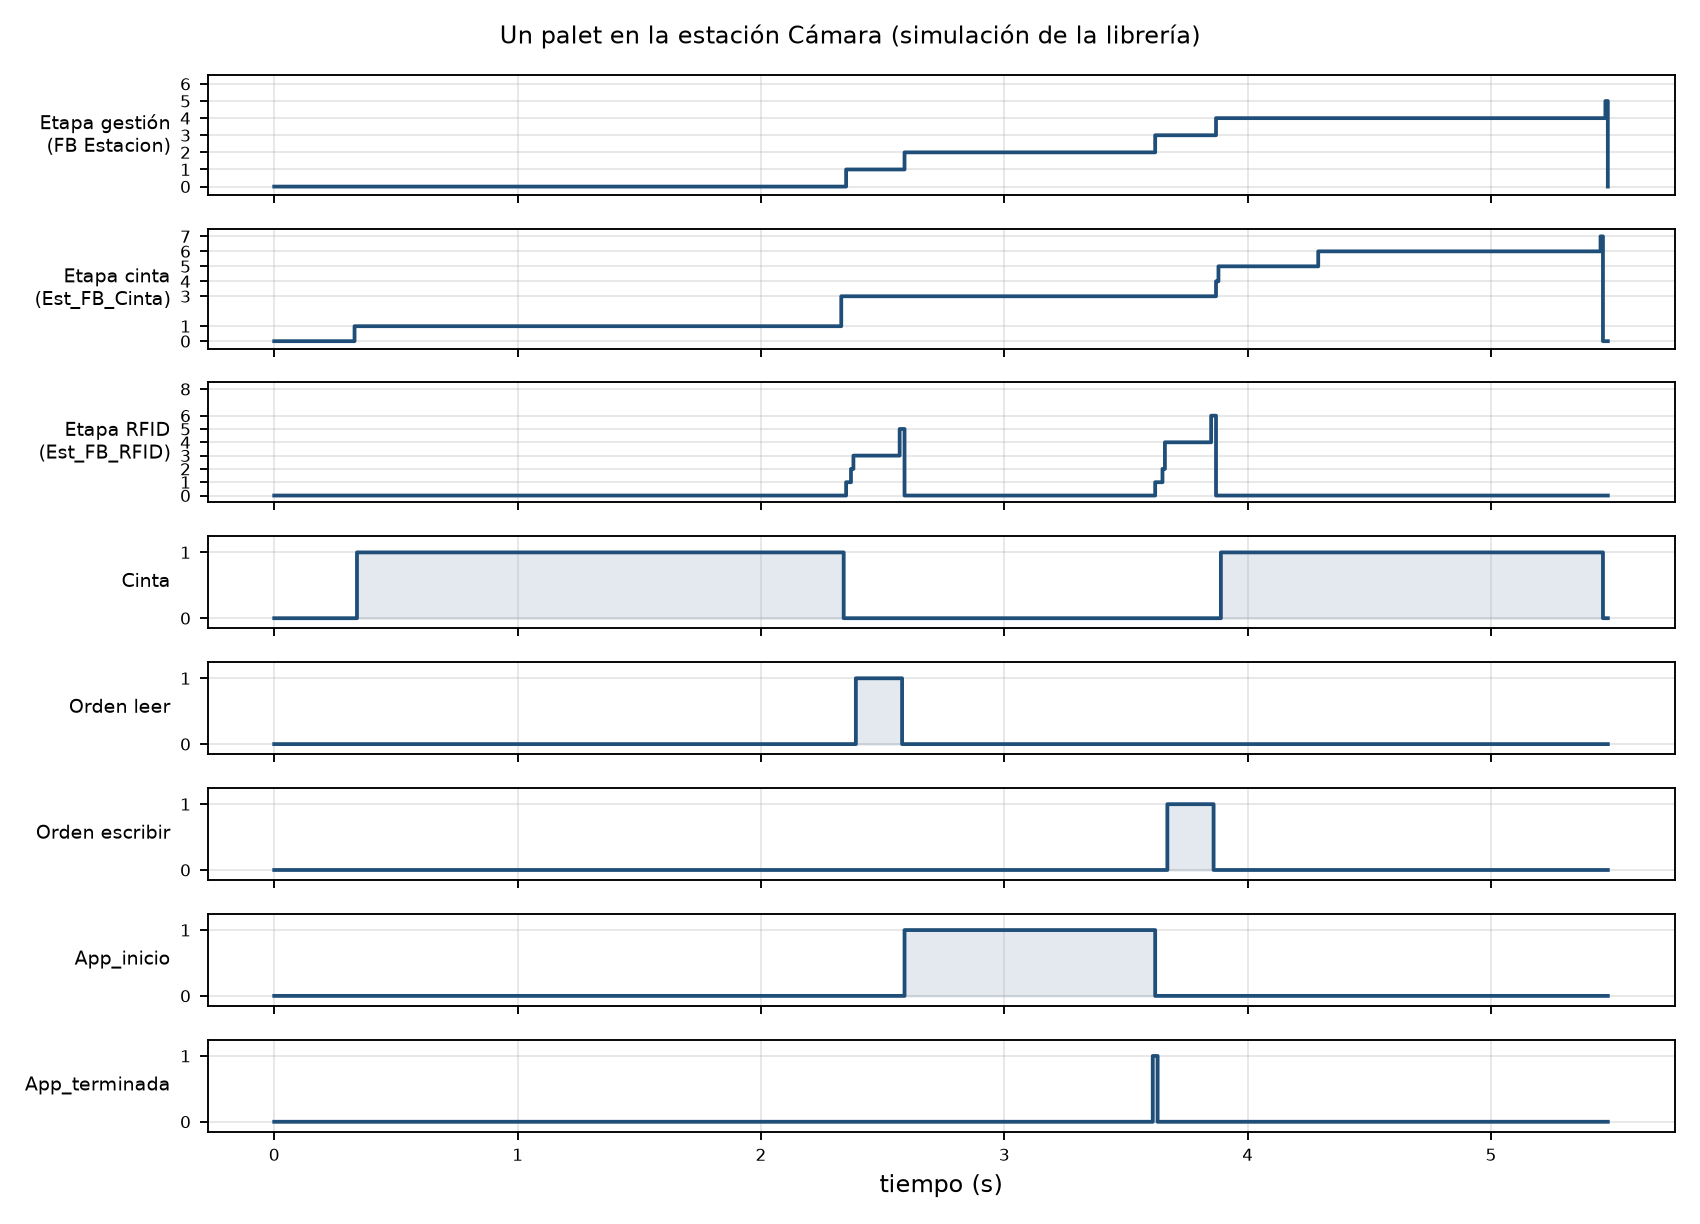
\includegraphics[width=\textwidth]{figuras/crono_ciclo_camara.png}
\caption{Un palet en la estación Cámara, simulación del código de la librería. De arriba abajo: etapa de la secuencia, etapa de la cinta, etapa del RFID, cinta en marcha, orden de leer, orden de escribir, \cod{App\_inicio} y \cod{App\_terminada}.}
\label{fig:crono}
\end{figure}

\section{Qué hay dentro del archivo de la librería}
El archivo \texttt{CPLabCore\_v\vlib.zal20} contiene dos cosas distintas, y conviene no confundirlas (la sección~\ref{sec:tipos-copias} explica la diferencia):

\begin{center}
\small
\begin{tabularx}{\textwidth}{>{\ttfamily\small}p{4.5cm}p{2.4cm}X}
\toprule
\textnormal{\textbf{Nombre}} & \textbf{Clase} & \textbf{Para qué sirve} \\
\midrule
\multicolumn{3}{l}{\sffamily\bfseries\color{azul} Tipos (con versión): lo que se usa tal cual} \\
Est\_FB\_Estacion & FB & La secuencia del palet; es lo único que llamas desde \cod{Main}. \\
Est\_FB\_Modo & FB & Botones, modos y emergencia. Lo llama \cod{Est\_FB\_Estacion}. \\
Est\_FB\_Cinta & FB & Cinta, stopper y recuento de palets. Lo llama \cod{Est\_FB\_Estacion}. \\
Est\_FB\_RFID & FB & Lector RFID. Lo llama \cod{Est\_FB\_Estacion}. \\
UDT\_Entradas\_Basico & UDT & Botonera y sensores de la cinta (módulo básico). \\
UDT\_Salidas\_Basico & UDT & Luces, cinta y stopper (módulo básico). \\
UDT\_Entradas\_Stopper & UDT & Sensores del módulo del stopper. \\
UDT\_Entradas\_RFID & UDT & Señales del lector RFID y los 28 bytes leídos. \\
UDT\_Salidas\_RFID & UDT & Órdenes al lector y los 28 bytes a escribir. \\
UDT\_Estado & UDT & Estado interno de la estación (modos, órdenes, errores). \\
\midrule
\multicolumn{3}{l}{\sffamily\bfseries\color{naranja!80!black} Copias maestras, carpeta \cod{Plantilla}: puntos de partida que copias y cambias} \\
Est\_FB\_App\_Plantilla & FB & Esqueleto vacío de aplicación, con el contrato ya hecho. \\
Main & OB & \cod{Main} de ejemplo con las dos llamadas cableadas. \\
DB\_Estacion & DB & Bloque de datos con las señales del contrato y la imagen. \\
Tabla de variables estándar & Tags & Los siete tags de E/S con su UDT y su dirección. \\
UDT\_Entradas\_APP, UDT\_Salidas\_APP & UDT & Ejemplo de E/S de aplicación (las de Out). \\
FB\_App\_Out, DB\_App\_out & FB, DB & La aplicación completa de la estación Out, como ejemplo. \\
\bottomrule
\end{tabularx}
\end{center}
